\documentclass[11pt]{article}
%Gummi|063|=)
\title{\textbf{The fabrik of knowledge}}
\usepackage{graphicx}
\usepackage{amsmath}
\begin{document}
\maketitle


\section{smallest part of what we call knowledge}
The picture shows an assemblage of concepts as they look when plotted with GraphViz.
Its a bit like snow as every concept has a different structure,
some simple ones some complex generally a concept can have one ore more 
exits which lead into one or more related concepts like\\
( I'm going = to the shop // crazy )



\begin{figure}[htp]
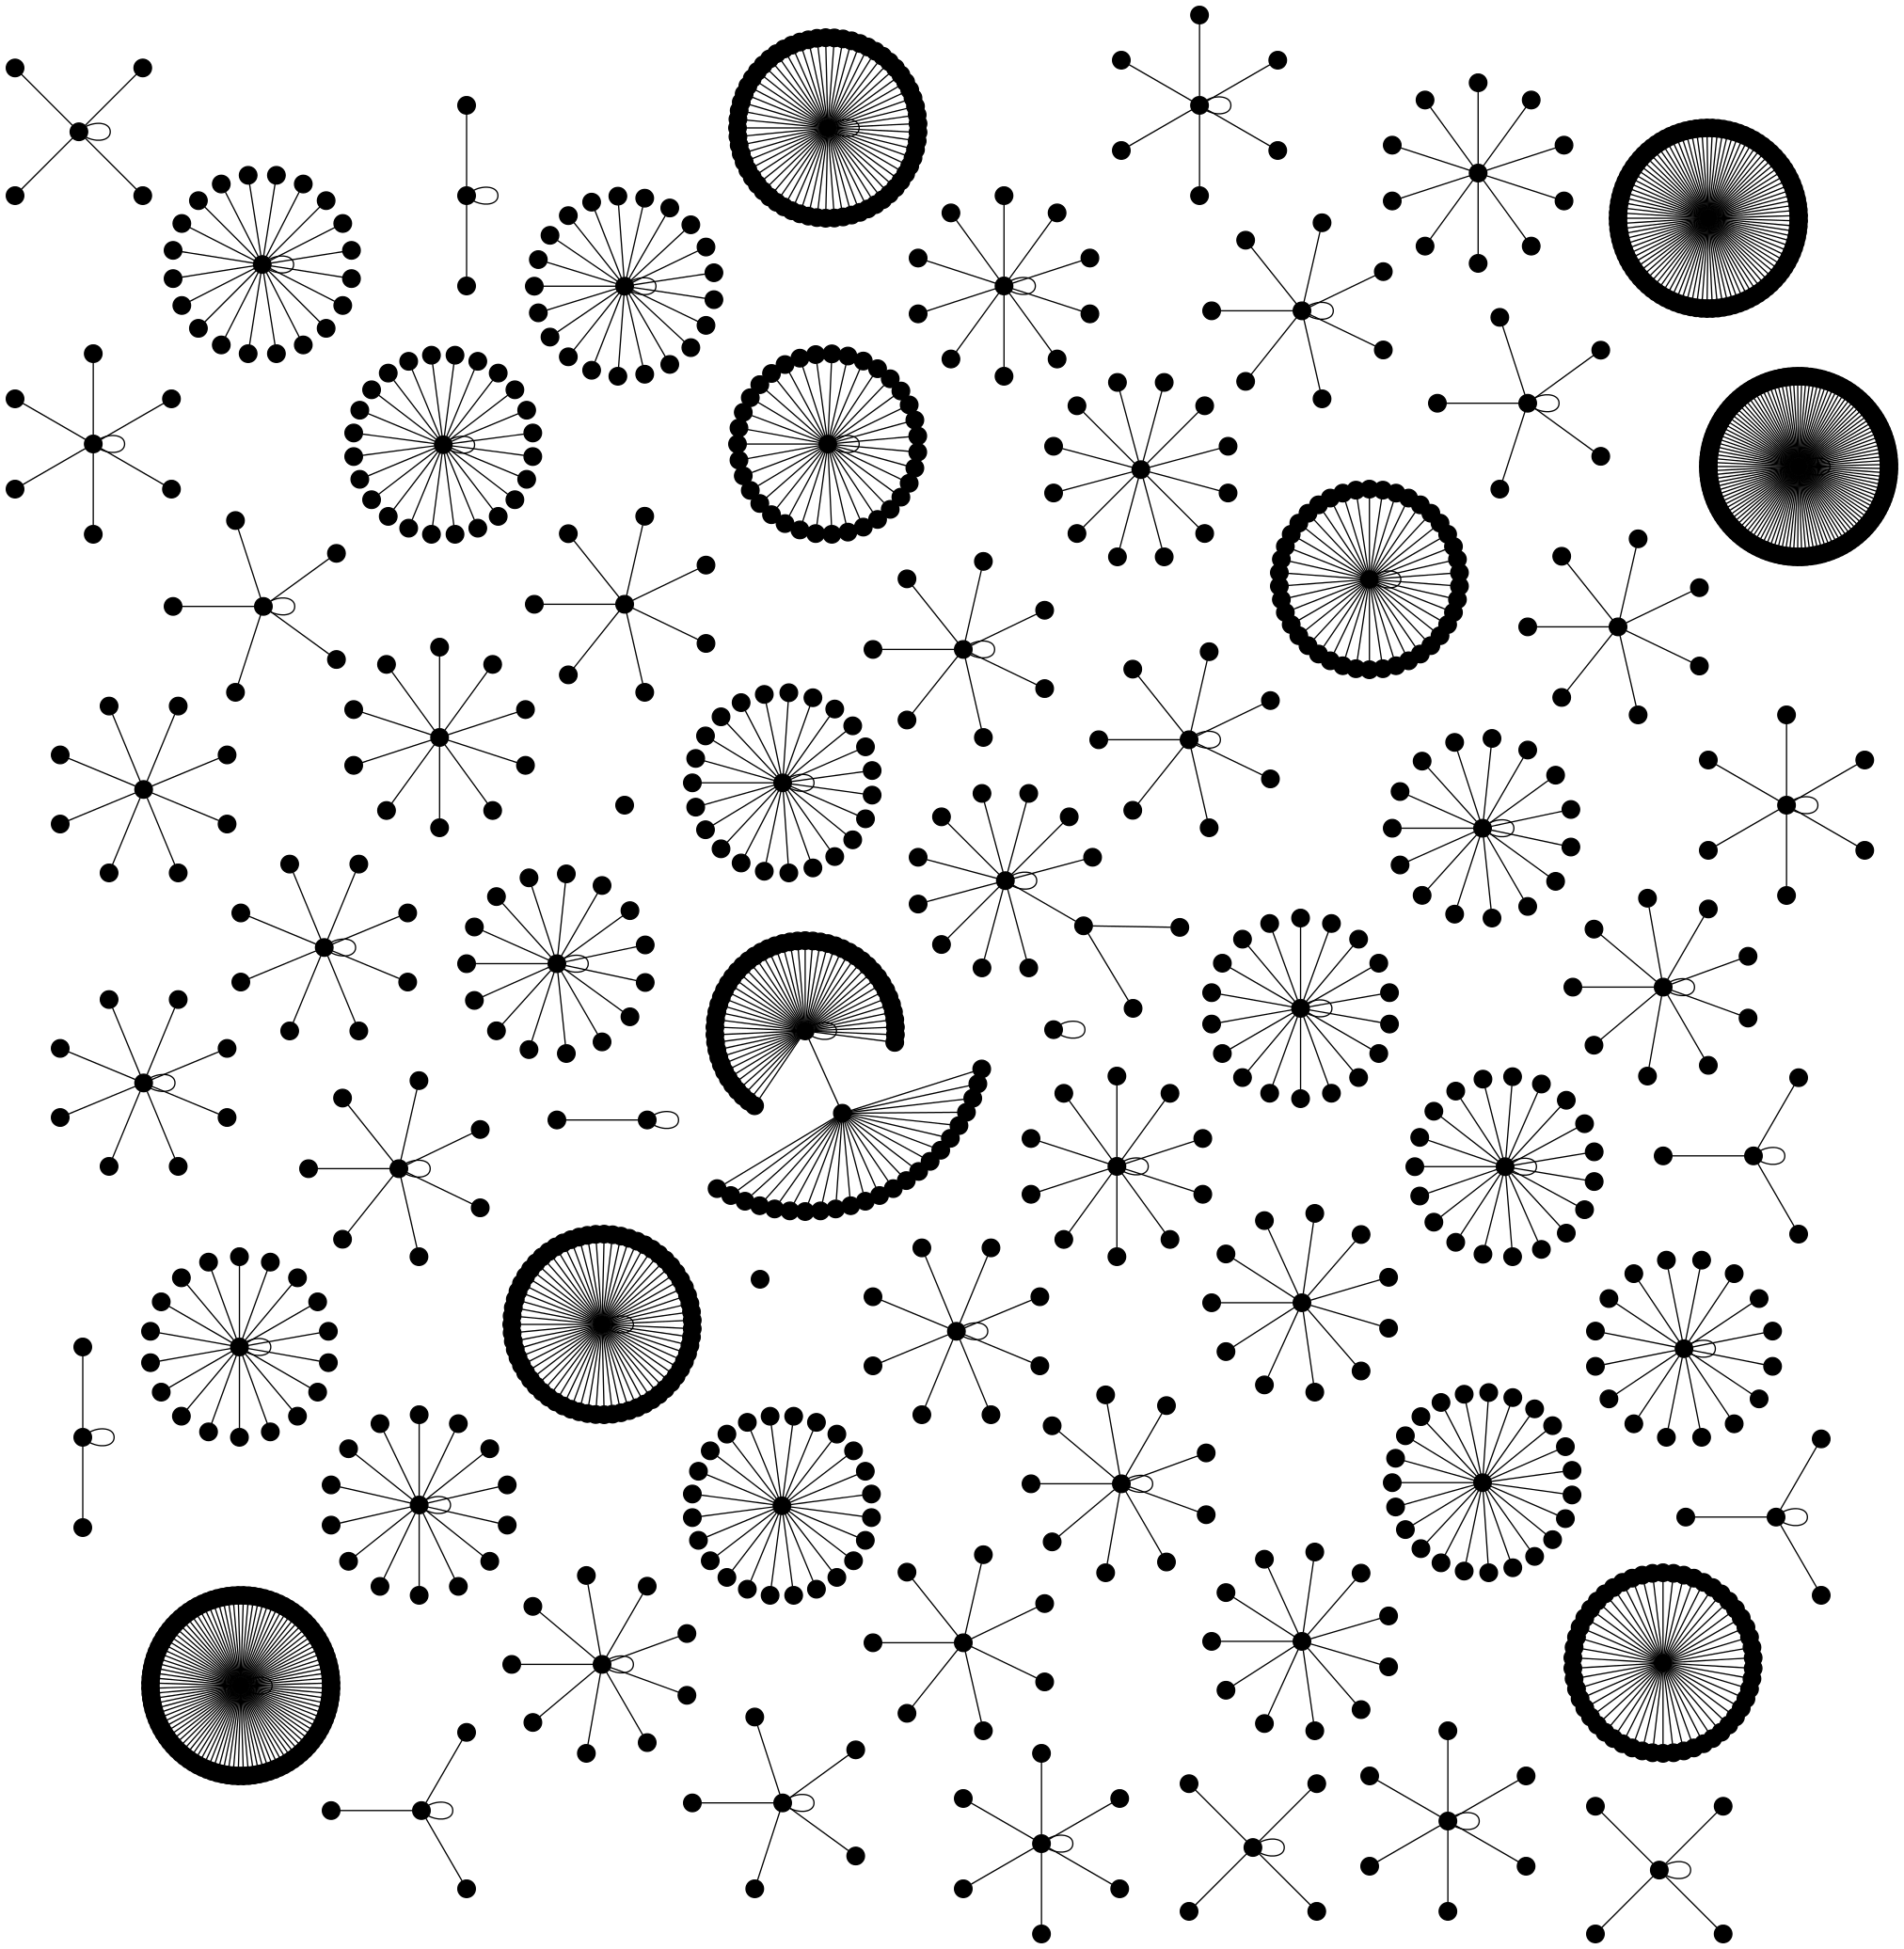
\includegraphics[scale=0.10]{img/w_directories.png}
\caption{a random generation of unrelated concepts}
\label{}
\end{figure}




\section{A knowledge system }

A large number of concepts even if assembled randomly 
will form a system where the relations will form connections 
which would make it possible to move from one concept to any other within 
the system.

\begin{figure}[htp]
\centering
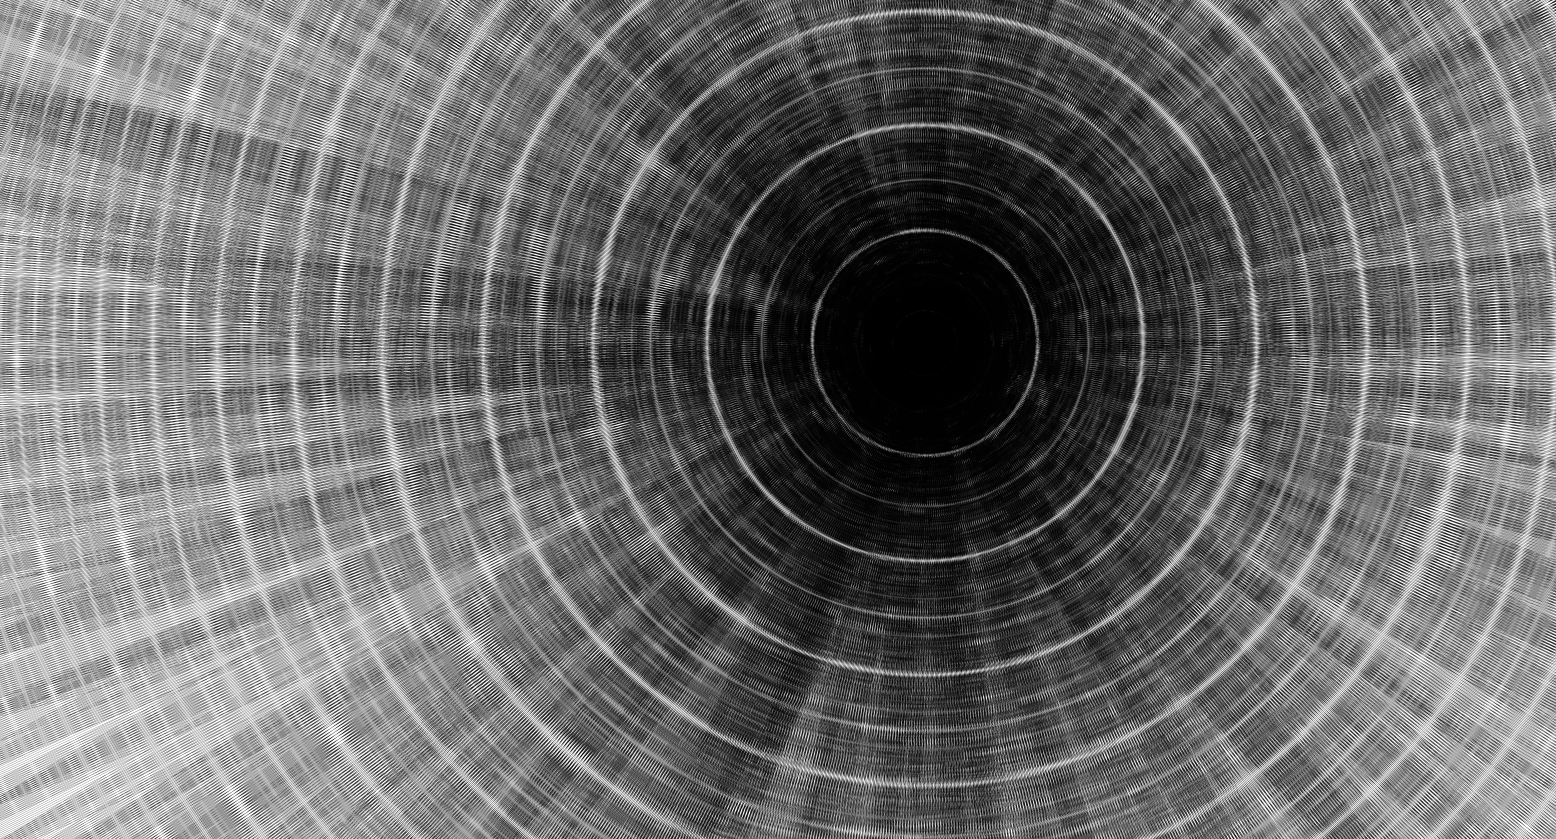
\includegraphics[scale=0.40]{img/1362924302_directories.png}
\caption{knowledge system with round about 1k concepts}
\label{every thought is interlocked somewhere at some point}
\end{figure}



\section{Making knowledge}
Lets start to render something simple like 
science-fiction


\begin{figure}[htp]
\centering
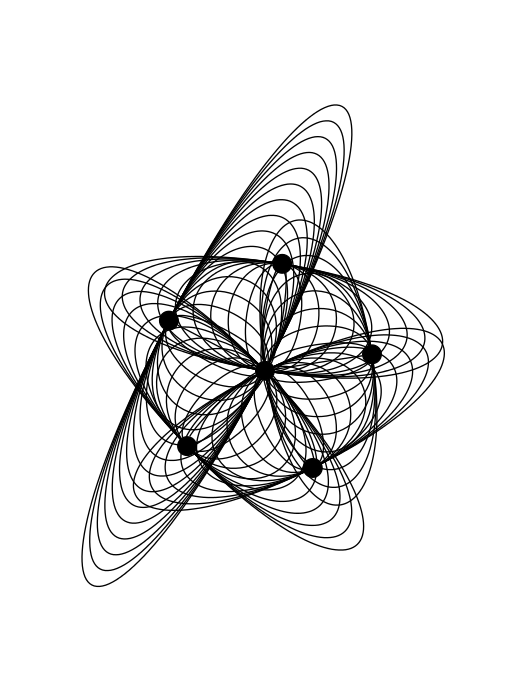
\includegraphics[scale=0.80]{img/science_fiction_directories.png}
\caption{}
\label{}
\end{figure}


\end{document}

